\documentclass[12pt]{article}

\usepackage[usenames]{color}
\usepackage{listings}
\usepackage{verbatim}
\usepackage{fancyhdr}
\usepackage{graphicx}
\usepackage{amssymb,amsthm}
%\usepackage[fleqn]{amsmath}
\usepackage{amsmath}
% \usepackage[final,notref,notcite,color]{showkeys}
\usepackage[left=1in,top=1in,right=1in,bottom=1in,letterpaper]{geometry}
\renewcommand{\baselinestretch}{1.2}

\pagestyle{fancy}
\lhead{}
\chead{}
\rhead{}
\lfoot{}
\cfoot{\thepage}
\rfoot{}



%% editing
\usepackage[shortlabels]{enumitem}
\usepackage[normalem]{ulem}

%% macros for commenting
\usepackage{mathtools}
\usepackage[normalem]{ulem} % to use \sout

%% math packages
% \usepackage{amsmath} % not needed for Springer
\usepackage{amssymb}
\usepackage{mathrsfs}

%\usepackage{subfigure}
%\usepackage{url}

%% a light-weight algorithm environment
\newtheorem{algo}{Algorithm}

%% highlighting and commenting
\newcommand{\outline}[1]{{\color{brown}#1}}
\newcommand{\rev}[1]{{\color{blue}#1}}
\newcommand{\remove}[1]{{\sout{#1}}}
\newcommand{\cut}[1]{{}}

%% macros for letters

\newcommand{\va}{{\mathbf{a}}}
\newcommand{\vb}{{\mathbf{b}}}
\newcommand{\vc}{{\mathbf{c}}}
\newcommand{\vd}{{\mathbf{d}}}
\newcommand{\ve}{{\mathbf{e}}}
\newcommand{\vf}{{\mathbf{f}}}
\newcommand{\vg}{{\mathbf{g}}}
\newcommand{\vh}{{\mathbf{h}}}
\newcommand{\vi}{{\mathbf{i}}}
\newcommand{\vj}{{\mathbf{j}}}
\newcommand{\vk}{{\mathbf{k}}}
\newcommand{\vl}{{\mathbf{l}}}
\newcommand{\vm}{{\mathbf{m}}}
\newcommand{\vn}{{\mathbf{n}}}
\newcommand{\vo}{{\mathbf{o}}}
\newcommand{\vp}{{\mathbf{p}}}
\newcommand{\vq}{{\mathbf{q}}}
\newcommand{\vr}{{\mathbf{r}}}
\newcommand{\vs}{{\mathbf{s}}}
\newcommand{\vt}{{\mathbf{t}}}
\newcommand{\vu}{{\mathbf{u}}}
\newcommand{\vv}{{\mathbf{v}}}
\newcommand{\vw}{{\mathbf{w}}}
\newcommand{\vx}{{\mathbf{x}}}
\newcommand{\vy}{{\mathbf{y}}}
\newcommand{\vz}{{\mathbf{z}}}
%
%\newcommand{\ta}{{\tilde{a}}}
%\newcommand{\tb}{{\tilde{b}}}
%\newcommand{\tc}{{\tilde{c}}}
%\newcommand{\td}{{\tilde{d}}}
%\newcommand{\te}{{\tilde{e}}}
%\newcommand{\tf}{{\tilde{f}}}
%\newcommand{\tg}{{\tilde{g}}}
%\newcommand{\th}{{\tilde{h}}}
%\newcommand{\ti}{{\tilde{i}}}
%\newcommand{\tj}{{\tilde{j}}}
%\newcommand{\tk}{{\tilde{k}}}
%\newcommand{\tl}{{\tilde{l}}}
%\newcommand{\tm}{{\tilde{m}}}
%\newcommand{\tn}{{\tilde{n}}}
%\newcommand{\to}{{\tilde{o}}}
%\newcommand{\tp}{{\tilde{p}}}
%\newcommand{\tq}{{\tilde{q}}}
%\newcommand{\tr}{{\tilde{r}}}
%\newcommand{\ts}{{\tilde{s}}}
%\newcommand{\tt}{{\tilde{t}}}
%\newcommand{\tu}{{\tilde{u}}}
%\newcommand{\tv}{{\tilde{v}}}
%\newcommand{\tw}{{\tilde{w}}}
%\newcommand{\tx}{{\tilde{x}}}
%\newcommand{\ty}{{\tilde{y}}}
%\newcommand{\tz}{{\tilde{z}}}

\newcommand{\vA}{{\mathbf{A}}}
\newcommand{\vB}{{\mathbf{B}}}
\newcommand{\vC}{{\mathbf{C}}}
\newcommand{\vD}{{\mathbf{D}}}
\newcommand{\vE}{{\mathbf{E}}}
\newcommand{\vF}{{\mathbf{F}}}
\newcommand{\vG}{{\mathbf{G}}}
\newcommand{\vH}{{\mathbf{H}}}
\newcommand{\vI}{{\mathbf{I}}}
\newcommand{\vJ}{{\mathbf{J}}}
\newcommand{\vK}{{\mathbf{K}}}
\newcommand{\vL}{{\mathbf{L}}}
\newcommand{\vM}{{\mathbf{M}}}
\newcommand{\vN}{{\mathbf{N}}}
\newcommand{\vO}{{\mathbf{O}}}
\newcommand{\vP}{{\mathbf{P}}}
\newcommand{\vQ}{{\mathbf{Q}}}
\newcommand{\vR}{{\mathbf{R}}}
\newcommand{\vS}{{\mathbf{S}}}
\newcommand{\vT}{{\mathbf{T}}}
\newcommand{\vU}{{\mathbf{U}}}
\newcommand{\vV}{{\mathbf{V}}}
\newcommand{\vW}{{\mathbf{W}}}
\newcommand{\vX}{{\mathbf{X}}}
\newcommand{\vY}{{\mathbf{Y}}}
\newcommand{\vZ}{{\mathbf{Z}}}

\newcommand{\cA}{{\mathcal{A}}}
\newcommand{\cB}{{\mathcal{B}}}
\newcommand{\cC}{{\mathcal{C}}}
\newcommand{\cD}{{\mathcal{D}}}
\newcommand{\cE}{{\mathcal{E}}}
\newcommand{\cF}{{\mathcal{F}}}
\newcommand{\cG}{{\mathcal{G}}}
\newcommand{\cH}{{\mathcal{H}}}
\newcommand{\cI}{{\mathcal{I}}}
\newcommand{\cJ}{{\mathcal{J}}}
\newcommand{\cK}{{\mathcal{K}}}
\newcommand{\cL}{{\mathcal{L}}}
\newcommand{\cM}{{\mathcal{M}}}
\newcommand{\cN}{{\mathcal{N}}}
\newcommand{\cO}{{\mathcal{O}}}
\newcommand{\cP}{{\mathcal{P}}}
\newcommand{\cQ}{{\mathcal{Q}}}
\newcommand{\cR}{{\mathcal{R}}}
\newcommand{\cS}{{\mathcal{S}}}
\newcommand{\cT}{{\mathcal{T}}}
\newcommand{\cU}{{\mathcal{U}}}
\newcommand{\cV}{{\mathcal{V}}}
\newcommand{\cW}{{\mathcal{W}}}
\newcommand{\cX}{{\mathcal{X}}}
\newcommand{\cY}{{\mathcal{Y}}}
\newcommand{\cZ}{{\mathcal{Z}}}

\newcommand{\ri}{{\mathrm{i}}}
\newcommand{\rr}{{\mathrm{r}}}

\newcommand{\EE}{{\mathbb{E}}}


%% macros for math notions and operators

\newcommand{\RR}{\mathbb{R}}
\newcommand{\CC}{\mathbb{C}}
\newcommand{\ZZ}{\mathbb{Z}}
\renewcommand{\SS}{{\mathbb{S}}}
\newcommand{\SSp}{\mathbb{S}_{+}}
\newcommand{\SSpp}{\mathbb{S}_{++}}
\newcommand{\sign}{\mathrm{sign}}
\newcommand{\vzero}{\mathbf{0}}
\newcommand{\vone}{{\mathbf{1}}}

\newcommand{\st}{{\text{s.t.}}} % subject to
\newcommand{\St}{{\mathrm{subject~to}}} % subject to
\newcommand{\op}{{\mathrm{op}}} % subscript for operator norm
\newcommand{\opt}{{\mathrm{opt}}} % subscript for optimal solution
%\newcommand{\supp}{{\mathrm{supp}}} % support
\newcommand{\Prob}{{\mathrm{Prob}}} % probability
\newcommand{\Diag}{{\mathrm{Diag}}} % vector -> diagonal matrix
%\newcommand{\diag}{{\mathrm{diag}}} % matrix diagonal -> vector
\newcommand{\dom}{{\mathrm{dom}}} % domain
\newcommand{\range}{{\mathrm{range}}} % domain
%\newcommand{\grad}{{\nabla}}    % gradient
\newcommand{\tr}{{\mathrm{tr}}} % trace
\newcommand{\TV}{{\mathrm{TV}}} % total variation
\newcommand{\Proj}{{\mathrm{Proj}}}
\newcommand{\prj}{{\mathrm{prj}}}
\newcommand{\prox}{\mathbf{prox}}
\newcommand{\refl}{\mathbf{refl}}
\newcommand{\reflh}{\refl^{\bH}}
\newcommand{\proxh}{\prox^{\bH}}
\newcommand{\minimize}{\text{minimize}}
\newcommand{\bgamma}{\boldsymbol{\gamma}}
\newcommand{\bsigma}{\boldsymbol{\sigma}}
\newcommand{\bomega}{\boldsymbol{\omega}}
\newcommand{\blambda}{\boldsymbol{\lambda}}
\newcommand{\bH}{\vH}
\newcommand{\bbH}{\mathbb{H}}
\newcommand{\bB}{\boldsymbol{\cB}}
\newcommand{\Tau}{\mathrm{T}}
\newcommand{\tnabla}{\widetilde{\nabla}}
\newcommand{\TDRS}{T_{\mathrm{DRS}}}
\newcommand{\TPRS}{T_{\mathrm{PRS}}}
\newcommand{\TFBS}{T_{\mathrm{FBS}}}
\newcommand{\best}{\mathrm{best}}
\newcommand{\kbest}{k_{\best}}
\newcommand{\diff}{\mathrm{diff}}
\newcommand{\barx}{\bar{x}}
\newcommand{\xgbar}{\bar{x}_g}
\newcommand{\xfbar}{\bar{x}_f}
\newcommand{\hatxi}{\hat{\xi}}
\newcommand{\xg}{x_g}
\newcommand{\xf}{x_f}
\newcommand{\du}{\mathrm{d}u}
\newcommand{\dy}{\mathrm{d}y}
\newcommand{\kconvergence}{\stackrel{k \rightarrow \infty}{\rightarrow }}
\DeclareMathOperator{\shrink}{shrink} % shrinkage
\DeclareMathOperator*{\argmin}{arg\,min}
\DeclareMathOperator*{\argmax}{arg\,max}
\DeclareMathOperator*{\Min}{minimize}
\DeclareMathOperator*{\Max}{maximize}
\DeclareMathOperator*{\Fix}{Fix}
\DeclareMathOperator*{\zer}{zer}
\DeclareMathOperator*{\nablah}{\nabla^{\bH}}
\DeclareMathOperator*{\gra}{gra}
\DeclarePairedDelimiter{\dotpb}{\langle}{\rangle_{\bH}}
\DeclarePairedDelimiter{\dotpv}{\langle}{\rangle_{\vH}}
\DeclarePairedDelimiter{\dotp}{\langle}{\rangle}

%% macros for environments math equations

\newcommand{\MyFigure}[1]{../fig/#1}

\newcommand{\bc}{\begin{center}}
\newcommand{\ec}{\end{center}}

\newcommand{\bdm}{\begin{displaymath}}
\newcommand{\edm}{\end{displaymath}}

\newcommand{\beq}{\begin{equation}}
\newcommand{\eeq}{\end{equation}}

\newcommand{\bfl}{\begin{flushleft}}
\newcommand{\efl}{\end{flushleft}}

\newcommand{\bt}{\begin{tabbing}}
\newcommand{\et}{\end{tabbing}}

\newcommand{\beqn}{\begin{align}}
\newcommand{\eeqn}{\end{align}}

\newcommand{\beqs}{\begin{align*}} % no equation numbers
\newcommand{\eeqs}{\end{align*}}  % no equation numbers
\def \la{\langle}
\def \ra{\rangle}
%% macros for theorem-like environments

%\newtheorem{theorem}{Theorem}
\newtheorem{assumption}{Assumption}
%\newtheorem{condition}{Condition}
%\newtheorem{rul}{Rule}
%\newtheorem{definition}{Definition}
%\newtheorem{corollary}{Corollary}
%\newtheorem{remark}{Remark}
%\newtheorem{lemma}{Lemma}
%\newtheorem{proposition}{Proposition}
%\newtheorem{example}{Example}
%\newtheorem{proof}{Proof}

\definecolor{mygreen}{RGB}{28,172,0} % color values Red, Green, Blue
\definecolor{mylilas}{RGB}{170,55,241}

%%%%%%%%%%%%%%%%%%%%%%%%%%%%%%%%%%%%%%%%%%%%%

\title{Final Project of MATP6610 }
\author{Shuting Yang RIN: 661967441}
\date{May-07-2021}

\begin{document}

\lstset{language=Matlab,%
    basicstyle=\footnotesize\ttfamily,
    breaklines=true,%
    morekeywords={matlab2tikz},
    deletekeywords={diff},
    keywordstyle=\color{blue},%
    %otherkeywords={self},             % Add keywords here
    identifierstyle=\color{black},%
    stringstyle=\color{mylilas},
    commentstyle=\color{mygreen},%
    showstringspaces=false,%without this there will be a symbol in the places where there is a space
    numbers=left,%
    numberstyle={\tiny \color{black}},% size of the numbers
    numbersep=9pt, % this defines how far the numbers are from the text
    %emph=[1]{for,end,break},emphstyle=[1]\color{red}, %some words to emphasise
    %emph=[2]{word1,word2}, emphstyle=[2]{style},
}

\maketitle


\vspace{0.2cm}


\section*{Topic I: Support Vector Machine }

\vskip 0.3cm
\noindent
{\bf Part 2}  \ The problem of soft-margin SVM, defined as

\begin{equation}\label{e1}
{\rm minimize}_{w,b,t}\sum\limits_{i=1}^{N}t_i+\frac{\lambda}{2}||w||^2,
\end{equation}
subject to
$$
y_i(w^Tx_i+b)\geq 1-t_i, \ t_i>0, \ i=1,2,\cdots,N
$$
is solved using the augmented Lagrangian Method (ALM).

\vskip 0.2cm
\noindent
We solve this inequality constraint problem by introducing slack variables $s_i, i=1,2,\cdots,N$, and convert it into an equality constraint. The soft-margin SVM problem then becomes 
\begin{equation}\label{e2}
{\rm minimize}_{w,b,t}(f(w,b,t)=\sum\limits_{i=1}^{N}t_i+\frac{\lambda}{2}||w||^2), \ {\rm s.t.}  \ g_i(w,b,t)+s_i=0, \ {\rm and} \ s_i\geq 0, i=1,2,\cdots,N,
\end{equation}
where $$
g_i(w,b,t)=1-t_i-y_i(w^Tx_i+b).
$$
Let $u\geq 0$ be the multiplier to $g_i+s_i$. The augmented Lagrangian function of (2) is
$$
{\mathcal L}_{\beta}(w,b,t,s,u)=f(w,b,t)+\sum\limits_{i=1}^N\left[u_i(g_i(w,b,t)+s_i)+\frac{\beta}{2}(g_i(w,b,t)+s_i)^2\right],
$$
i.e.,
$$
{\mathcal L}_{\beta}(w,b,t,s,u)=\sum\limits_{i=1}^{N}t_i+\frac{\lambda}{2}||w||^2
+\sum\limits_{i=1}^N\left[u_i(1-t_i-y_i(w^Tx_i+b)+s_i)+\frac{\beta}{2}(1-t_i-y_i(w^Tx_i+b)+s_i)^2\right],
$$
by Quadratic Penalty.

\vskip 0.2cm
\noindent
An iterative approach of the ALM requires us to solve the following subproblems at the $k$-th iteration:
\begin{equation}\label{e3}
w^{(k+1)}={\rm argmin}_{w}{\mathcal L}_{\beta}(w,b^{(k)},t^{(k)},s^{(k)},u^{(k)})
\end{equation}
\begin{equation}\label{e4}
b^{(k+1)}={\rm argmin}_b{\mathcal L}_{\beta}(w^{(k)},b,t^{(k)},s^{(k)},u^{(k)})
\end{equation}
\begin{equation}\label{e5}
t^{(k+1)}={\rm argmin}_{t}{\mathcal L}_{\beta}(w^{(k)},b^{(k)},t,s^{(k)},u^{(k)})
\end{equation}
\begin{equation}\label{e6}
s^{(k+1)}={\rm argmin}_{s}{\mathcal L}_{\beta}(w^{(k)},b^{(k)},t^{(k)},s,u^{(k)})
\end{equation}
And the multiplier $u$ is updated as 
$$
u_i^{(k+1)}=u_i^{(k)}+\beta(g_i(w^{(k)},b^{(k)},t^{(k)})+s_i^{(k)}), \ i=1,2,\cdots,N.
$$
Applying the Projected Gradient Method, we need to solve the following problems at the $k$-th iteration:
\begin{equation}\label{e7}
w^{(k+1)}={\rm Proj}_{w\in{\mathbb R}^p}(w^{(k,\beta)}-\alpha_k\nabla_w{\mathcal L}_{\beta}) 
\end{equation}
\begin{equation}\label{e8}
b^{(k+1)}={\rm Proj}_{b\in{\mathbb R}}(b^{(k,\beta)}-\alpha_k\nabla_b{\mathcal L}_{\beta})
\end{equation}
\begin{equation}\label{e9}
t^{(k+1)}={\rm Proj}_{t\in{\mathbb R}^N}(t^{(k,\beta)}-\alpha_k\nabla_t{\mathcal L}_{\beta})
\end{equation}
\begin{equation}\label{e10}
s^{(k+1)}={\rm Proj}_{s\in{\mathbb R}^N}(s^{(k,\beta)}-\alpha_k\nabla_s{\mathcal L}_{\beta}).
\end{equation}
To choose an appropriate step size $\alpha$ in each of the subproblems (\ref{e7}), (\ref{e8}), (\ref{e9}), and (\ref{e10}), a Backtracking Line Search method (Algorithm 3.1 of textbook) is applied. 

\vskip 0.2cm
\noindent
Use the update of $w$ as an example. 

\vskip 0.2cm
\noindent
Treating all other variables as constants.

\vskip 0.2cm
\noindent
Choose
$$\bar{\alpha}>0, \  \rho\in (0,1),  \ c\in(0,1);
$$
Set 
$$
\alpha \leftarrow \bar{\alpha};$$
Repeat until
$$
{\mathcal L}_{\beta}(w+\alpha p_k)\leq {\mathcal L}_{\beta}(w)+c\alpha\nabla{\mathcal L}_{\beta}^T\cdot p_k.
$$
$$
\alpha_k\leftarrow \bar{\alpha}
$$
End repeat.\\
Terminate $\alpha_k=\alpha$.

\vskip 0.3cm
\noindent
{\bf Part 3}. \ Using this Backtracking Line Search Method, the step size $\alpha$ for each of the subproblems (\ref{e7}), (\ref{e8}), (\ref{e9}), and (\ref{e10}) can be found. Apart from the above stopping condition used in Line Search, the other two stopping conditions used in solving the subproblems in (\ref{e7}), (\ref{e8}), (\ref{e9}), and (\ref{e10}) are gradient error (grad-err) and maximum iterations. The project gradient method for solving $w, b, t, s$ will stop if grad-err is less than the tolerance (sub-tol) of $10^{-3}$. The stopping conditions of the outer loop are max(dual violation, primal violation) $\leq$ tolerance and maximum iteration time. 

Specifically, when solving for $w,b,t$, and $s$, we set the gradients in the following (\ref{e11})-(\ref{e14}) to zero to meet the optimality condition.
\begin{equation}\label{e11}
\nabla_{w}{\mathcal L}_{\beta}=\lambda w-\sum\limits_{i=1}^Nu_iy_ix_i-\beta\sum\limits_{i=1}^N(1-t_i-y_i(w^Tx_i+b)+s_i)y_ix_i
\end{equation} 
\begin{equation}\label{e12}
\nabla_{b}{\mathcal L}_{\beta}=-\sum\limits_{i=1}^Nu_iy_i-\beta\sum\limits_{i=1}^Ny_i(1-t_i-y_i(w^Tx_i+b)+s_i)
\end{equation} 
\begin{equation}\label{e13}
\nabla_{t_i}{\mathcal L}_{\beta}=1-u_i-\beta(1-t_i-y_i(w^Tx_i+b)+s_i), \ i=1,2,\cdots, N
\end{equation} 
\begin{equation}\label{e14}
\nabla_{s_i}{\mathcal L}_{\beta}=u_i+\beta(1-t_i-y_i(w^Tx_i+b)+s_i), \ s_i\geq 0, \ i=1,2,\cdots, N.
\end{equation}
\vskip 0.2cm
\noindent 
To derive the dual feasibility and primal feasibility, we need to consider the KKT conditions.
$$
\left\{
\begin{array}{l}
\nabla f+\sum\limits_{i=1}^Nu_ig_i=\overrightarrow{0} \ \ ({\rm dual \  feasibility})\\
1-t_i-y_i(w^Tx_i+b)+s_i=0 \\
s_i\geq 0\\
g_i\leq 0\\
u_ig_i=0, \ i=1,2,\cdots, N. 
\end{array}
\right.
$$
The violation of primary feasibility is 
$$
\varphi_i^{(k)}=1-t_i-y_ib+s_i-y_ix_i^Tw^{(k)}, \ i=1,2,\cdots,N.
$$
By update rules of $u_i$, 
$$
u_i^{(k+1)}=u_i^{(k)}+\beta(1-t_i-y_i(w^Tx_i+b)).
$$
The optimality conditions for each of  (\ref{e3})-(\ref{e6}) holds at 
$$
w^{(k+1)}: \ \nabla_w{\mathcal L}_{\beta}(w^{(k+1)}, b^{(k)}, t^{(k)}, s^{(k)}, u^{(k)})=\overrightarrow{0}
$$
$$
b^{(k+1)}: \ \nabla_b{\mathcal L}_{\beta}(w^{(k)}, b^{(k+1)}, t^{(k)}, s^{(k)}, u^{(k)})=\overrightarrow{0}
$$
$$
t^{(k+1)}: \ \nabla_t{\mathcal L}_{\beta}(w^{(k)}, b^{(k)}, t^{(k+1)}, s^{(k)}, u^{(k)})=\overrightarrow{0}
$$
$$
s^{(k+1)}: \ \nabla_s{\mathcal L}_{\beta}(w^{(k)}, b^{(k)}, t^{(k)}, s^{(k+1)}, u^{(k)})=\overrightarrow{0}.
$$
Replacing the $u_i$ in the above equations, we get
\begin{equation}\label{e15}
\lambda w^{(k+1)}-\sum\limits_{i=1}^Nu_i^{(k+1)}y_ix_i-2\beta\sum\limits_{i=1}^N(1-t_i-y_i(w^Tx_i+b)+s_i)y_ix_i=\overrightarrow{0}
\end{equation}
\begin{equation}\label{e16}
-\sum\limits_{i=1}^Nu_i^{(k+1)}y_i=0
\end{equation}
\begin{equation}\label{e17}
1-u_i^{(k+1)}=0
\end{equation}
\begin{equation}\label{e18}
u_i^{(k+1)}=0
\end{equation}
Comparing (\ref{e15})-(\ref{e18}) with (\ref{e11})-(\ref{e14}), we derive the violation of dual feasibility as follows:
$$
||\beta\sum\limits_{i=1}^N(1-t_i-y_i(w^Tx_i+b)+s_i)y_ix_i||+||\sum\limits_{i=1}^N(1-t_i-y_i(w^Tx_i+b)+s_i)||
+2||\beta\sum\limits_{i=1}^N(1-t_i-y_i(w^Tx_i+b)+s_i)||.
$$
$$
$$
The testing results are in the pages following.
$$
$$

\newpage
\section*{Part 4-5: SVM-spam Test Result and Figures}
$$
$$
Using a \(\beta\) = 0.5 and \(\lambda\) = 1 for ALM; c = 0.3 and dec-ratio = 0.5 for parameters in line search, the testing result for SVM-spam is as follows. Considering the length of print, the following printing result only included 20 outer iterations. Note that the classification result is satisfactory, but the computational time is long, which implies that the solver efficiency can be improved.
\begin{verbatim}
>> test_model_SVM_spam
Testing by student code

out iter = 1, pres = 1.5913e+01, dres = 7.7029e+03, subit = 20
out iter = 2, pres = 1.9653e+01, dres = 7.2852e+03, subit = 20
out iter = 3, pres = 2.4659e+01, dres = 6.9207e+03, subit = 20
out iter = 4, pres = 2.9430e+01, dres = 6.6608e+03, subit = 20
out iter = 5, pres = 3.3975e+01, dres = 6.4147e+03, subit = 20
out iter = 6, pres = 3.8469e+01, dres = 6.1799e+03, subit = 20
out iter = 7, pres = 4.2963e+01, dres = 5.9699e+03, subit = 20
out iter = 8, pres = 4.7484e+01, dres = 5.8101e+03, subit = 20
out iter = 9, pres = 5.2063e+01, dres = 5.6763e+03, subit = 20
out iter = 10, pres = 5.6713e+01, dres = 5.5477e+03, subit = 20
out iter = 11, pres = 6.1445e+01, dres = 5.4226e+03, subit = 20
out iter = 12, pres = 6.6201e+01, dres = 5.2982e+03, subit = 20
out iter = 13, pres = 7.0988e+01, dres = 5.1773e+03, subit = 20
out iter = 14, pres = 7.5842e+01, dres = 5.0672e+03, subit = 20
out iter = 15, pres = 8.0834e+01, dres = 4.9793e+03, subit = 20
out iter = 16, pres = 8.5810e+01, dres = 4.8936e+03, subit = 20
out iter = 17, pres = 9.0873e+01, dres = 4.8193e+03, subit = 20
out iter = 18, pres = 9.6033e+01, dres = 4.7560e+03, subit = 20
out iter = 19, pres = 1.0120e+02, dres = 4.6913e+03, subit = 20
out iter = 20, pres = 1.0641e+02, dres = 4.6273e+03, subit = 20
Running time is 7.5966
classification accuracy on testing data: 80.87%

Testing by instructor code

out iter = 1, pres = 5.8762e+01, dres = 1.2285e+02, subit = 20
out iter = 2, pres = 5.6312e+01, dres = 1.7191e+02, subit = 20
out iter = 3, pres = 5.2984e+01, dres = 2.9018e+02, subit = 20
out iter = 4, pres = 4.9673e+01, dres = 4.2253e+02, subit = 20
out iter = 5, pres = 4.5763e+01, dres = 6.1716e+02, subit = 20
out iter = 6, pres = 4.1862e+01, dres = 4.0074e+02, subit = 20
out iter = 7, pres = 3.6981e+01, dres = 5.7551e+02, subit = 20
out iter = 8, pres = 3.2761e+01, dres = 7.5702e+02, subit = 20
out iter = 9, pres = 2.7349e+01, dres = 6.3044e+02, subit = 20
out iter = 10, pres = 2.1775e+01, dres = 5.7407e+02, subit = 20
out iter = 11, pres = 1.6240e+01, dres = 6.6476e+02, subit = 20
out iter = 12, pres = 1.1068e+01, dres = 6.8514e+02, subit = 20
out iter = 13, pres = 8.7292e+00, dres = 7.2352e+02, subit = 20
out iter = 14, pres = 3.9052e+00, dres = 5.4746e+02, subit = 20
out iter = 15, pres = 3.0713e+00, dres = 6.9758e+02, subit = 20
out iter = 16, pres = 2.2853e+00, dres = 7.1635e+02, subit = 20
out iter = 17, pres = 1.9643e+00, dres = 6.0396e+02, subit = 20
out iter = 18, pres = 1.4222e+00, dres = 4.6273e+02, subit = 20
out iter = 19, pres = 8.2589e-01, dres = 4.2048e+02, subit = 20
out iter = 20, pres = 5.1938e-01, dres = 3.7364e+02, subit = 20
Running time is 1.2367
classification accuracy on testing data: 78.87%
\end{verbatim}
$$
$$

\section*{Part 4: SVM-rho02 Test Result}
$$
$$
Using a \(\beta\) = 0.05 and \(\lambda\) = 0.1 for ALM; c = 0.2 and dec-ratio = 0.5 for parameters in line search, the testing result for SVM-rho02 is as follows. Considering the length of print, the following printing result only included 20 outer iterations. Note that the classification result is satisfactory. But the computational time is also long, which implies that the solver efficiency can be improved.
\begin{verbatim}
>> test_model_SVM_rho02
Testing by student code

out iter = 1, pres = 6.0296e+02, dres = 3.7561e+04, subit = 20
out iter = 2, pres = 6.2264e+02, dres = 3.5346e+04, subit = 20
out iter = 3, pres = 6.4119e+02, dres = 3.3164e+04, subit = 20
out iter = 4, pres = 6.5899e+02, dres = 3.1088e+04, subit = 20
out iter = 5, pres = 6.7609e+02, dres = 2.9114e+04, subit = 20
out iter = 6, pres = 6.9252e+02, dres = 2.7238e+04, subit = 20
out iter = 7, pres = 7.0830e+02, dres = 2.5453e+04, subit = 20
out iter = 8, pres = 7.2348e+02, dres = 2.3756e+04, subit = 20
out iter = 9, pres = 7.3808e+02, dres = 2.2144e+04, subit = 20
out iter = 10, pres = 7.5212e+02, dres = 2.0612e+04, subit = 20
out iter = 11, pres = 7.6563e+02, dres = 1.9158e+04, subit = 20
out iter = 12, pres = 7.7864e+02, dres = 1.7781e+04, subit = 20
out iter = 13, pres = 7.9117e+02, dres = 1.6475e+04, subit = 20
out iter = 14, pres = 8.0323e+02, dres = 1.5238e+04, subit = 20
out iter = 15, pres = 8.1484e+02, dres = 1.4068e+04, subit = 20
out iter = 16, pres = 8.2603e+02, dres = 1.2958e+04, subit = 20
out iter = 17, pres = 8.3680e+02, dres = 1.1909e+04, subit = 20
out iter = 18, pres = 8.4716e+02, dres = 1.0920e+04, subit = 20
out iter = 19, pres = 8.5711e+02, dres = 9.9894e+03, subit = 20
out iter = 20, pres = 8.6667e+02, dres = 9.1170e+03, subit = 20
Running time is 2.3713
classification accuracy on testing data: 91.00%

Testing by instructor code

out iter = 1, pres = 0.0000e+00, dres = 2.1968e+00, subit = 20
out iter = 2, pres = 0.0000e+00, dres = 1.1382e+00, subit = 20
out iter = 3, pres = 0.0000e+00, dres = 2.3946e-01, subit = 20
out iter = 4, pres = 0.0000e+00, dres = 2.1082e-01, subit = 20
out iter = 5, pres = 0.0000e+00, dres = 1.9195e-01, subit = 20
out iter = 6, pres = 0.0000e+00, dres = 1.7443e-01, subit = 20
out iter = 7, pres = 1.8128e-03, dres = 1.5715e-01, subit = 20
out iter = 8, pres = 0.0000e+00, dres = 1.4038e-01, subit = 20
out iter = 9, pres = 0.0000e+00, dres = 1.2686e-01, subit = 20
out iter = 10, pres = 5.7565e-04, dres = 1.1427e-01, subit = 20
out iter = 11, pres = 6.7911e-04, dres = 1.0713e-01, subit = 20
out iter = 12, pres = 0.0000e+00, dres = 9.6717e-02, subit = 20
out iter = 13, pres = 3.6957e-04, dres = 9.1574e-02, subit = 20
out iter = 14, pres = 5.3285e-04, dres = 8.7507e-02, subit = 20
out iter = 15, pres = 9.0454e-04, dres = 8.2353e-02, subit = 20
out iter = 16, pres = 4.6719e-04, dres = 7.7391e-02, subit = 20
out iter = 17, pres = 0.0000e+00, dres = 7.3662e-02, subit = 20
out iter = 18, pres = 9.7905e-04, dres = 7.3561e-02, subit = 20
out iter = 19, pres = 4.5927e-04, dres = 6.7546e-02, subit = 20
out iter = 20, pres = 3.5000e-06, dres = 6.5227e-02, subit = 20
Running time is 0.3918
classification accuracy on testing data: 95.00%
\end{verbatim}
$$
$$

\section*{Part 4: SVM-rho08 Test Result}
$$
$$
Using a \(\beta\) = 0.2 and \(\lambda\) = 0.1 for ALM; c = 0.45 and dec-ratio = 0.5 for parameters in line search, the testing result for SVM-rho08 is as follows. Considering the length of print, the following printing result only included 20 outer iterations. Note that the classification result is not very satisfactory. The computational time is also long, which implies that the solver efficiency can be improved.
\begin{verbatim}
>> test_model_SVM_rho08
Testing by student code

out iter = 1, pres = 4.2137e+02, dres = 5.4505e+04, subit = 20
out iter = 2, pres = 4.2648e+02, dres = 3.3706e+04, subit = 20
out iter = 3, pres = 4.2896e+02, dres = 2.2022e+04, subit = 20
out iter = 4, pres = 4.3298e+02, dres = 1.4830e+04, subit = 20
out iter = 5, pres = 4.3743e+02, dres = 1.0156e+04, subit = 20
out iter = 6, pres = 4.4197e+02, dres = 7.0361e+03, subit = 20
out iter = 7, pres = 4.4638e+02, dres = 4.8796e+03, subit = 20
out iter = 8, pres = 4.5069e+02, dres = 3.3364e+03, subit = 20
out iter = 9, pres = 4.5495e+02, dres = 2.2667e+03, subit = 20
out iter = 10, pres = 4.5914e+02, dres = 1.5177e+03, subit = 20
out iter = 11, pres = 4.6329e+02, dres = 1.0144e+03, subit = 20
out iter = 12, pres = 4.6742e+02, dres = 6.8076e+02, subit = 20
out iter = 13, pres = 4.7159e+02, dres = 4.7717e+02, subit = 20
out iter = 14, pres = 4.7581e+02, dres = 3.4866e+02, subit = 20
out iter = 15, pres = 4.8013e+02, dres = 2.6447e+02, subit = 20
out iter = 16, pres = 4.8454e+02, dres = 2.2514e+02, subit = 20
out iter = 17, pres = 4.8874e+02, dres = 1.5442e+02, subit = 4
out iter = 18, pres = 4.9309e+02, dres = 1.4545e+02, subit = 4
out iter = 19, pres = 4.9751e+02, dres = 1.4145e+02, subit = 4
out iter = 20, pres = 5.0202e+02, dres = 1.3577e+02, subit = 4
Running time is 1.8118
classification accuracy on testing data: 68.00%

Testing by instructor code

out iter = 1, pres = 0.0000e+00, dres = 2.0617e+00, subit = 20
out iter = 2, pres = 0.0000e+00, dres = 1.1143e+00, subit = 20
out iter = 3, pres = 4.1960e-04, dres = 9.6344e-01, subit = 20
out iter = 4, pres = 0.0000e+00, dres = 8.0175e-01, subit = 20
out iter = 5, pres = 4.7455e-04, dres = 6.8857e-01, subit = 20
out iter = 6, pres = 4.7980e-03, dres = 5.5524e-01, subit = 20
out iter = 7, pres = 1.4519e-03, dres = 5.0271e-01, subit = 20
out iter = 8, pres = 0.0000e+00, dres = 4.3816e-01, subit = 20
out iter = 9, pres = 0.0000e+00, dres = 3.7695e-01, subit = 20
out iter = 10, pres = 0.0000e+00, dres = 3.5100e-01, subit = 20
out iter = 11, pres = 0.0000e+00, dres = 3.3167e-01, subit = 20
out iter = 12, pres = 0.0000e+00, dres = 3.1579e-01, subit = 20
out iter = 13, pres = 4.7800e-04, dres = 3.0103e-01, subit = 20
out iter = 14, pres = 3.0787e-03, dres = 2.9638e-01, subit = 20
out iter = 15, pres = 0.0000e+00, dres = 2.8099e-01, subit = 20
out iter = 16, pres = 2.3343e-03, dres = 2.7290e-01, subit = 20
out iter = 17, pres = 4.4062e-04, dres = 2.5993e-01, subit = 20
out iter = 18, pres = 1.5581e-03, dres = 2.5460e-01, subit = 20
out iter = 19, pres = 6.9371e-04, dres = 2.5084e-01, subit = 20
out iter = 20, pres = 8.7837e-04, dres = 2.4451e-01, subit = 20
Running time is 0.2020
classification accuracy on testing data: 80.50%
\end{verbatim}
The output figures of SVM-spam, SVM-rho02 and SVM-08 are in the pages following.

% to include your figure
\begin{figure}\caption{SVM-spam}
\begin{center}
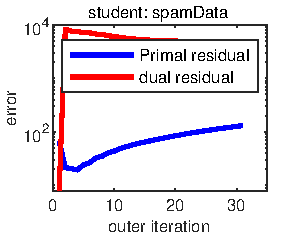
\includegraphics[width=0.8\textwidth]{student_spam.pdf} 
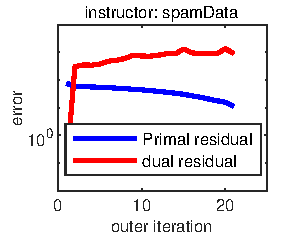
\includegraphics[width=0.8\textwidth]{instructor_spam.pdf} 
\end{center}
\end{figure}

% to include your figure
\begin{figure}\caption{SVM-rho02}
\begin{center}
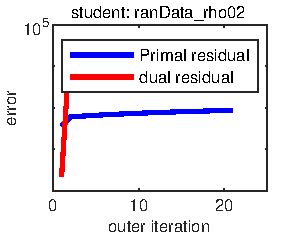
\includegraphics[width=0.8\textwidth]{student_rho02.pdf} 
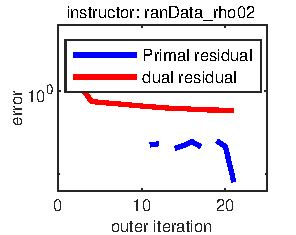
\includegraphics[width=0.8\textwidth]{instructor_rho02.pdf} 
\end{center}
\end{figure}

% to include your figure
\begin{figure}\caption{SVM-rho08}
\begin{center}
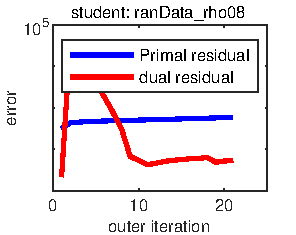
\includegraphics[width=0.8\textwidth]{student_rho08.pdf} 
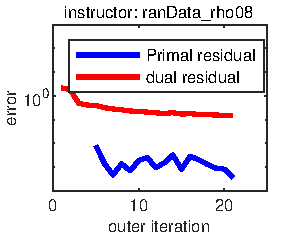
\includegraphics[width=0.8\textwidth]{instructor_rho08.pdf} 
\end{center}
\end{figure}

\newpage
\section*{Topic II(Bonus)}

We use alternating minimization method. Let
$$
L(x,y,v)=\frac{1}{2}||XY-M||_{F}^2+\sum\limits_{i=1}^{r}[v_i(\sum\limits_{j=1}^{n}Y_{ij}-1)+\frac{\beta}{2}(\sum\limits_{j=1}^{n}Y_{ij}-1)^2], \ \beta>0.
$$
The problem is to solve
$$
{\rm minimize}_{X,Y}L(X,Y,v)
$$
Let
$$
f(X,Y)=\frac{1}{2}||XY-M||_{F}^2, \ h_i(X,Y)=\sum\limits_{j=1}{n}Y_{ij}-1.
$$
Dual feasibility for $X$:
$$
\nabla_Xf(X,Y)+\sum\limits_{i=1}^{r}u_i\nabla_Xh_i(X,Y)=\nabla_Xf(X,Y)=0.
$$
Dual feasibility for $Y$:
$$
\nabla_Y f(X,Y)+\sum\limits_{i=1}^ru_i\nabla_Yh_i(X,Y)=0.
$$
Primary feasibility:
$$
 h_i(X,Y)=\sum\limits_{j=1}^{n}Y_{ij}-1=0, \ i=1,2,\cdots,r.
$$

\end{document}
